\documentclass[a4,titlepage]{jsreport}
% \usepackage{samplebox}
\usepackage[dvipdfmx]{graphicx}
\usepackage{fancyvrb}

\title{KLIC 講習会テキスト\\KLIC システム編}
\date{\ }
\author{平成5年12月~~財団法人 新世代コンピュータ技術開発機構~~作成
\\平成7年9月~~財団法人 日本情報処理開発協会開発研究室~~改訂}

\tolerance5000
\begin{document}
\renewcommand{\textfraction}{0.2}
\renewcommand{\topfraction}{0.7}
\renewcommand{\bottomfraction}{0.7}
\renewcommand{\floatpagefraction}{0.7}
\addtolength{\textheight}{27pt}
\addtolength{\topmargin}{-18pt}

\makeatletter
\let\savedchap\@makechapterhead
\def\@makechapterhead{\vspace*{-1cm}\savedchap}
\makeatletter

\maketitle

\chapter*{はじめに}

\bgroup\large
本編は KLIC 講習会のために作成した KLIC システム利用法の入門テキスト
である.

KLIC システムの基本的な使い方, トレーサを使ってのデバッグ法と, KLIC シ
ステムのインストール方法について解説した.

講習会テキストとしては, 別に「KL1 言語編」がある.  こちらは KLIC 言語
の仕様とプログラミング・テクニックの基本を解説したものである.  本編と
合わせて御利用願いたい.

\begin{flushright}
1993年12月\\
ICOT KLIC 開発グループ\\
1995年9月\\
JIPDEC KLIC 保守普及グループ\\
\end{flushright}
\egroup
\thispagestyle{empty}

\newpage
\setcounter{page}{0}
\pagenumbering{roman}
\tableofcontents

\chapter{KLICの使い方}
\setcounter{page}{0}
\pagestyle{plain}
\pagenumbering{arabic}

この章では, KLICシステムの基本的な使い方について説明する.  

\section{KLICシステムの作り}
KLICは, 基本的に, 

\begin{quote}
KL1で書かれたプログラムをCにコンパイルすることにより実行可能コードを
作る
\end{quote}
システムである.  但し, 手で, KL1$\Rightarrow$Cコンパイラを立ち上げ, 
次にCコンパイラを立ち上げ$\ldots$とするのは, 面倒なので, 
\verb|klic|というコマンドを起動するのみでKL1のコンパイル, Cのコンパイル/
リンクを行なうことができる.  

\section{まず, 走らせよう!}
なにはともあれ, KLICシステムを走らせ, 実際にプログラムを動かしてみよう.  

KL1プログラムをコンパイルするためには, 

% \begin{samplebox}
\begin{Verbatim}[frame=single]
% klic `KL1プログラムのファイル名'
\end{Verbatim}
% \end{samplebox}
とすればよい (KL1プログラムのファイル名には, 拡張子\verb|`.kl1'|をつけ
ること).
例えば, 図\ref{fig:nrev0}に示す
\verb|nrev0.kl1|というプログラムをコンパイルするためには, 

% \begin{samplebox}
\begin{Verbatim}[frame=single]
% klic nrev0.kl1
\end{Verbatim}
% \end{samplebox}
とする.  この\verb|klic|コマンドを実行すると, 実行形式のファイルが
作成され, オプションを何も指定しないと (指定の仕方は後述) 
このファイルは\verb|a.out|という名前になる.  
また, \verb|nrev0.kl1|をコンパイルした結果できた
Cプログラムも同じディレクトリに\verb|nrev0.c|という
ファイル名で作成されている.  

この実行形式ファイルを実行すれば, KL1プログラムを実行することができる.  
% \begin{samplebox}
\begin{Verbatim}[frame=single]
% a.out
[6,5,4,3,2,1]
\end{Verbatim}
% \end{samplebox}

\section{KL1プログラムの構成}
では, KL1プログラムの構成を見てみよう (図\ref{fig:nrev0}参照).

\begin{figure}[htbp]
\begin{center}
\leavevmode
\begin{minipage}{12.5cm}
% \begin{center}
% \begin{samplebox}
\begin{Verbatim}[frame=single,baselinestretch=0.8]
% nrev0.kl1
% リストを逆転する.  
:- module main.

main :- true |
    nrev([1,2,3,4,5,6],X),
    io:outstream([print(X),nl]).

nrev([], Y) :- true | Y=[].
nrev([A|X], Y) :- true |
     nrev(X, RevX),
     append(RevX, [A], Y).

append([], Y, Z) :- true  | Y = Z.
append([A|X], Y, Z) :- true |
     Z=[A|Z1], append(X, Y, Z1).
\end{Verbatim}
% \end{samplebox}
% \end{center}
\end{minipage}
\end{center}
\caption{nrev0.kl1}
\label{fig:nrev0}
\end{figure}

まず, 最初に\verb|:- module main.|と書かれているが, これは
モジュール宣言と呼ばれるものである (詳細はのちほど説明する).  まずは, 
KL1プログラムの最初は必ず
\verb|:- module main.|と書いておけば良い, と理解しておけば良い.  

次に, \verb|main :- ...| と書かれているが, これは, 述語\verb|main|
を定義していることを表す.  
\verb|klic|コマンドでコンパイルしてできたコードは, 
まず, この述語\verb|main|を実行する決まりになっている.  したがって, KLIC
システムで利用するためのKL1プログラムには必ずこの述語\verb|main|が
存在する必要がある (必ずしもファイルの先頭で定義されている必要はない).  
「本当に行ないたいこと (今回であれば, \verb|nrev([1,2,3,4,5,6],X)|という
述語)」はこの述語\verb|main|から呼び出されるようにしておけば良い.  

また, \verb|io:outstream([print(X),nl])| とあるのは, 
項\verb|X|を標準出力に印字するための述語呼出しであり, 
あらかじめシステムで用意されていものである.  
述語\verb|io:outstream(Stream)|は, 
\verb|Stream|に流れて来るメッセージに従い, 標準出力に
印字を行う.  
今回は, 以下の2種類のメッセージを利用している.  

\begin{itemize}
\item \verb|print/1| $\ldots$ 引数の項全体が具体化するまで待ち, 
印字する.  

\item \verb|nl/0| $\ldots$ 標準出力に改行コードを送る.  
\end{itemize}

これで, 簡単なKL1プログラムを書いて, \verb|klic|コマンドでコンパイルし, 
実行できるようになった.  

\section{もうちょっと複雑な使い方}
先に述べた方法では, 1つのファイルをコンパイルすることしかできず, 
少し大きなプログラムを書こうと思うと, 少々面倒である.  
また, 必ず, \verb|a.out|という実行形式のファイルができてしまう.  
ここでは, もうちょっと複雑な\verb|klic|コマンドの使い方を
解説する.  

\subsection{klicコマンドの仕組みを少し}
先程も説明したように, \verb|klic|コマンドによって, KL1プログラムはCに
コンパイルされ, 実行形式になる.  これをもう少し詳しく見ると, 
図\ref{fig:klicflow}のようになる.  

\begin{figure}
\begin{center}
% \epsfile{file=klicflow.eps,width=.8\textwidth}
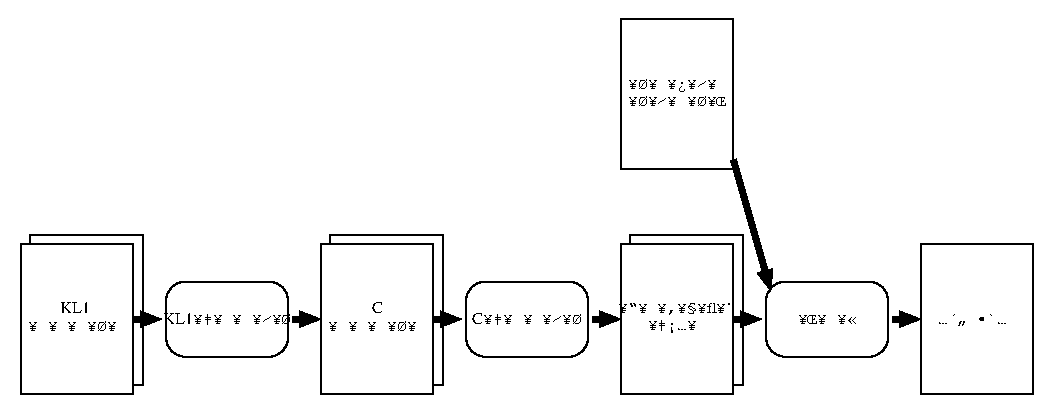
\includegraphics[width=.8\textwidth]{fig/klicflow.eps}
\end{center}
\caption{klicコマンドの仕組み}
\label{fig:klicflow}
\end{figure}

\verb|klic|コマンドは, 以下のようなプログラムを呼び出す.  

\begin{description}
\item[KL1 $\Rightarrow$ Cコンパイラ:\ ]
KL1をCに変換するコンパイラ.  
このコンパイラは KL1 言語で記述されている.  KLICシステムの心臓部分である.  

\item[Cコンパイラ:\ ]
上のKL1コンパイラが生成したCのコードをオブジェクトコードにする.  

\item[リンカ:\ ]
Cコンパイラが生成したオブジェクトコード
\footnote{もちろん, KL1コンパイラが生成したCをコンパイルした
オブジェクトコードでなくとも, 
さらにはCコンパイラではなく, ほかのコンパイラで
生成されたオブジェクトコードであってもリンクをすることは
原理的には可能である.  }
とKL1プログラムが必要とする
ランタイム・ライブラリも併せてリンクする.  
もちろん, ここで複数のオブジェクトコードをリンクしても構わない.  
\end{description}

\subsection{2つのファイルの同時コンパイル/リンク}
では, \verb|klic|コマンドを使って2つのKL1プログラムを
同時にコンパイルし, 1つの実行形式にリンクしてみよう.  

先ほどの {\tt nrev0.kl1} と同じ内容のプログラムを2つのファイルに分けた
ものが {\tt nrev1.kl1} と {\tt append.\linebreak[1]kl1} である (図
\ref{fig:bar}参照).  この場合, 以下のようなコマンドにより1つの実行形式
ファイルを得ることができる.

% \begin{samplebox}
\begin{Verbatim}[frame=single]
% klic -o nrev nrev1.kl1 append.kl1
\end{Verbatim}
% \end{samplebox}

\verb|-o nrev|という指定は, 「実行形式のファイル名は\verb|nrev|とせよ」
ということを表す.  なにも指定しないと, (先ほどのように) \verb|a.out|
という名前のファイルが作成されてしまうが, この\verb|-o|オプション
を利用することによって実行形式のファイル名を自由に指定することができる.  

\subsection{モジュール}
では, 2つのファイルを見てみよう (図\ref{fig:bar}参照).  

\begin{figure}
\begin{center}
\begin{minipage}{7cm}
% \begin{samplebox}
\begin{Verbatim}[frame=single,baselinestretch=0.8]
:- module main.

main :- true |
    nrev([1,2,3,4,5,6], X),
    io:outstream([print(X),nl]).

nrev([], Y) :- true | Y = [].
nrev([A|X], Y) :- true |
    nrev(X, RevX),
    app:append(RevX, [A], Y).
\end{Verbatim}
% \end{samplebox}
\begin{center}
ファイル nrev1.kl1
\end{center}
\end{minipage}
% \hspace{1cm}
\hfil
\begin{minipage}{7.5cm}
% \begin{samplebox}
\begin{Verbatim}[frame=single,baselinestretch=0.8]
:- module app.

append([], Y, Z) :- true | Y = Z.
append([A|X], Y, Z) :- true |
    Z=[A|Z1], append(X, Y, Z1).
\end{Verbatim}
% \end{samplebox}
\begin{center}
ファイル append.kl1
\end{center}
\end{minipage}
\caption{nrev1.kl1, append.kl1}
\label{fig:bar}
\end{center}
\vspace*{-18pt}
\end{figure}

まず, \verb|nrev1.kl1|の先頭には\verb|:- module main.|と書かれているのは先程の
プログラムと同様である.  また, 述語\verb|main|も同様に定義されている.  
最後に, \verb|app:append(...)|と書かれているのに注意すること.  

次に\verb|append.kl1|を見ると最初には\verb|:- module app.|と書かれており, 
先程の記述とは異なっている.  

KL1では複数のファイルに定義された述語を互いに利用することができる.  
しかしながら, いくつものファイルを別々に記述すると, 
気がつかないうちに複数のファイルで同じ述語名が使われる可能性がある.  
これは, どの述語を呼び出すべきか分からなくなるので都合が悪い.  

KLICシステムで使用できるKL1プログラムは{\bf モジュール}という単位で
複数の述語を1まとめにすることができる.  
通常は1つのファイルが1つの
モジュールとなる.  
モジュールにはあとで区別できるように名前を
つけておく必要がある (この名前を{\bf 「モジュール名」}という).  
実は, 先頭にある \verb|:- module main|という宣言は, 
「このファイルのモジュール名は\verb|main|だよ」ということを宣言していたので
あった.  

ほかのモジュールの述語を呼び出そうとする場合には, その呼び出し先の
述語にモジュール名も添える必要がある.

\begin{center}
\begin{minipage}{6cm}
\begin{Verbatim}[frame=single]
 モジュール名:述語
\end{Verbatim}
\end{minipage}
\end{center}

たとえば, モジュール {\tt app} の述語 {\tt append(...)} を他のモジュー
ルから呼び出すためには, {\tt app:\linebreak[1]append(...)} とすれば良
い.  これで, どのモジュールに定義された述語を呼び出そうとしているのか
を明確にすることができる.  したがって, 同じ名前 (で違う動作をするよう
な) 述語を複数のモジュールで定義してしまっても, 区別がすることができる.

この「モジュール」の取扱はklicシステム
で最初に呼び出される述語についても同様である.  
「klicで最初に呼び出される述語は述語\verb|main|」
であることを既に説明したが, これは若干不正確で, 
実はモジュール\verb|main|にある述語\verb|main|を呼び出すことになっている.  

モジュールについて整理すると, 以下のようになる.  

\begin{itemize}
\item KL1のプログラムはファイル毎に「モジュール」と呼ばれる
述語の集合よりなる.  

\item 「モジュール」には名前をつける必要があり, それを「モジュール名」
という.  モジュールの先頭で, ``\verb|:- module|'' 宣言をすることで, 
モジュール名を指定する.

\item 他のモジュールで定義されている述語を呼び出すには, ``呼び出す述
語が定義されているモジュール名\verb|:|述語名'' と書く.

\item 最初に呼び出される述語は ``\verb|main:main|'' である.  
\end{itemize}

\subsection{分割コンパイルの方法}

先の使い方では「複数のファイルに対して同時に」コンパイル/リンクを行なっていた.  
しかしながら, 実際にある程度大きなプログラムを作成し, 
デバッグ/修正を繰り返すようになると, 
「複数のファイルのうち1つだけ」
を直してコンパイルし, それ以外のファイルのコンパイル結果 (オブジェクト
コード) とリンクしたくなるような場面に遭遇することが少なくない.  
\verb|klic|コマンドではそのような使い方をすることも可能である.  
以下のようにすれば, 別々にコンパイルし, 作成されたオブジェクトコードを
リンクすることができる.  

% \begin{samplebox}
\begin{Verbatim}[frame=single,baselinestretch=0.8]
% klic -c nrev1.kl1
% klic -c append.kl1
% klic -o nrev nrev1.o append.o
\end{Verbatim}
% \end{samplebox}

ここで, \verb|-c|というオプションは, 実行形式は作成せず, 
オブジェクトコードまでしか作成しないことを指定している.  
通常, \verb|klic|コマンドはなにも指定しなければ, 実行形式まで作成する 
(リンカまで起動する) ようになっているが, ここでリンクを行なっても, 
所詮, プログラムの全てが与えられていないので, 実行形式を
作成することができない.  そこで, オブジェクトコード (.o) の作成で
止める必要がある.  このオプションはそのために用いる.  
つまり, \verb|-c|と指定した時には, オブジェクトのコードを作成したところで
処理を止め, リンクを抑制する.  

しかしながら, 実際には, \verb|klic|コマンドは
ファイルの作成された日付を見て, コンパイルを行なう必要があるかどうか
\footnote{オブジェクトコードよりも, ソースコードの方が新しければ, 
最後に行なったコンパイル以降にソースコードが変更されていることに
なるので, コンパイルが行なわれる.  さもなくば, コンパイルを
行なう必要はない.  }を自動的に判断する機能 (UNIXの {\tt make} 
コマンドと同じ機能) を備えているので, 以下の
コマンドにより, 自動的に最小限の処理が行なわれる.  

% \begin{samplebox}
\begin{Verbatim}
% klic foo.kl1 bar.kl1
\end{Verbatim}
% \end{samplebox}

ここで, \verb|klic|コマンドが行なっていることを調べてみよう.  
\verb|-v|というオプションを使うと, 途中行なっている処理の様子を
見ることができる.  

% \begin{samplebox}
% {\small
\begin{Verbatim}[frame=single,baselinestretch=0.8]
%klic -o nrev -v nrev1.kl1 append.kl1
KLIC compiler driver version 1.513 (Thu Dec  8 11:55:54 JST 1994)
/usr/local/lib/klic/kl1cmp nrev1.kl1 </dev/null
/usr/local/lib/klic/kl1cmp append.kl1 </dev/null
/usr/local/lib/klic/klicdb  -X /usr/local/lib nrev1.ext append.ext
gcc -c  -o nrev1.o -I/usr/local/include -I. nrev1.c
gcc -c  -o append.o -I/usr/local/include -I. append.c
gcc -c  -o atom.o -I/usr/local/include -I. atom.c
gcc -c  -o funct.o -I/usr/local/include -I. funct.c
gcc -c  -o predicates.o -I/usr/local/include -I. predicates.c
gcc -o nrev atom.o funct.o predicates.o nrev1.o append.o -L/usr/local/lib -lklict \
-L/usr/lib -L/lib   -lm
%
\end{Verbatim}
% \end{samplebox}
% }

\subsection{KLICシステムについてさらにもう少し}

ここで, KLICシステムが作成するファイルについて説明を行なう.  

klicを動かしたあとのディレクトリを見ると, \verb|klic.db|や, 
\verb|atom.h|とかいった, 作った覚えのないファイルができているのを発見
するであろう.  
これらのファイルの働きについて解説する.  

\subsubsection{「記号」の扱い}

KL1のプログラムでは「アトム」や「ファンクタ」と呼ばれる「記号」が
数多く使われる.  例えば, 図\ref{fig:atomFunc}に示す
プログラムでは, \verb|foo|, \verb|bar|
といったアトム, \verb|foo/1|というファンクタが用いられている.  

\begin{figure}
\begin{center}
\begin{minipage}{6cm}
% \begin{samplebox}
\begin{Verbatim}[frame=single]
p(foo(X)) :- true | X=bar.
\end{Verbatim}
% \end{samplebox}
\end{minipage}
\caption{アトムとファンクタ}
\label{fig:atomFunc}
\end{center}
\end{figure}

これらは目で見た所, 明らかに「文字列」である.  しかしながら, 
これらの記号を内部的にも文字列として扱うことは, 利用するメモリの量や, 
速度 (たとえば, 文字列``bar''と, ``bal''が違うことを見るためには, 
3文字を1つづつ比較しなければなならない) の面で不利になる.  
そこで, KLICシステムでは, これらの「記号」は内部的には全て
「番号」で持っている.  例えば, ``foo''であれば104番, ``bar''であれば253番
$\ldots$と内部では変換されているのである.  
この変換はKLICの出力コードを効率化するため, コンパイル時に
全て行なわれる.  

さらにトレースやエラー表示のためには述語の印刷イメージを生成する
ための表も必要とする.

KLICシステムで作成されたプログラムはKL1の項を読んだり
書いたりすることができるが, その時にもこの記号$\Leftrightarrow$
番号の変換が行なわれる.  つまり, 項が読み込まれる時には
内部的な番号に置き換えられ, 項を出力する時には, 
番号を記号に置き換え, 人間に分かりやすく出力することができる.  

\subsubsection{複数ファイルでの「記号」の処理}
さて, ここで1つ問題がある.  

先にもあげたように, KLICシステムでは, 複数のKL1モジュールを
1つづつ別々にコンパイルすることができる.  
これらのモジュールの間では「記号」がやりとりされることは
当然考えられる.  しかしながら, 前章で説明したように, 
処理の効率を良くするため, 「記号」は, 内部では番号として扱われており, 
しかもコンパイルを行なう際に変換してしまう.  
モジュールの間で「記号」は受け渡されるので, 
異なったモジュールであっても同じ「記号」は同じ番号として
変換される必要が生じる.  「``foo''という記号はこのモジュールでは104番だけど, 
あのモジュールでは253番で, それはそのモジュールの``bar''という記号の
番号と同じになった」などということが起きてもらっては困るのである.  

この問題の解決のために用いられているのが, \verb|klic.db|
というファイルである.  
このファイルの中には, 
「どの記号はどの番号に変換されたか」が記録されている.  
KL1コンパイラは記号を見付けるたびに, このファイルにすでに登録されているか
どうか調べ, すでに登録されていれば, その番号に変換するようにしている.  
登録されていなければ (他に, まだ, コンパイルを行なっていない, 
同じ記号を使っているKL1プログラムがあるかも知れないので) 
そのファイルに「この記号は何番に変換したよ」ということを残しておく.  
つまり, このファイルを介して, 複数のKL1コンパイラが記号$\Leftrightarrow$
番号の変換規則をやりとりしているわけである.  

ファイル\verb|klic.db|は, 「KLICデータベース管理システム」
(\verb|klicdb|) というプログラムで管理されている.  
このプログラムにより
\verb|atom.h|, \verb|funct.h|なるファイルも生成され
KLICコンパイラが生成したCプログラム内に取り込まれることにより
記号$\Rightarrow$番号の変換がCコンパイル時に行なわれる.  

この\verb|klic.db|に書かれている情報は, 
KLICシステムで作られたプログラムが実行される時も
必要であるため, Cプログラムに変換され, コンパイル/リンクされる.  
これが, \verb|atom.c|, \verb|funct.c|, \verb|predicates.c|といったファ
イルである. 

従って, KLICシステムを使って, 複数のプログラムを作成してコンパイル/
プログラム修正を繰り返している時に, ここで挙げたファイルが無くなってしまうと, 
それ以降の処理はおかしくなることがある.  以下であげるファイルは
作った覚えがないからといって, 消してしまってはならない.  
\footnote{完成した実行形式のファイルはこれらのファイルを参照することは
ないので, その実行形式ファイルだけをどこかにコピーしてしまっても構わない.  }

\begin{itemize}
\item *.ext (.kl1と同じbasenameで拡張子が.ext)
\item klic.db
\item atom.c atom.h
\item funct.c funct.h
\item predicates.c
\end{itemize}

もし, 消してしまった場合は, {\tt -R} という強制再コンパイルオプションで
\verb|.kl1|プログラムをコンパイルし直すようにすれば, 
これらのファイルはまた生成される.  

この記号のメンテナンス関連の処理も含めたklicシステム全体の
ファイル/処理の流れを図\ref{fig:flow2}に示す.  

\begin{figure}
\begin{center}
% \epsfile{file=klicflow2.eps,width=.9\textwidth}
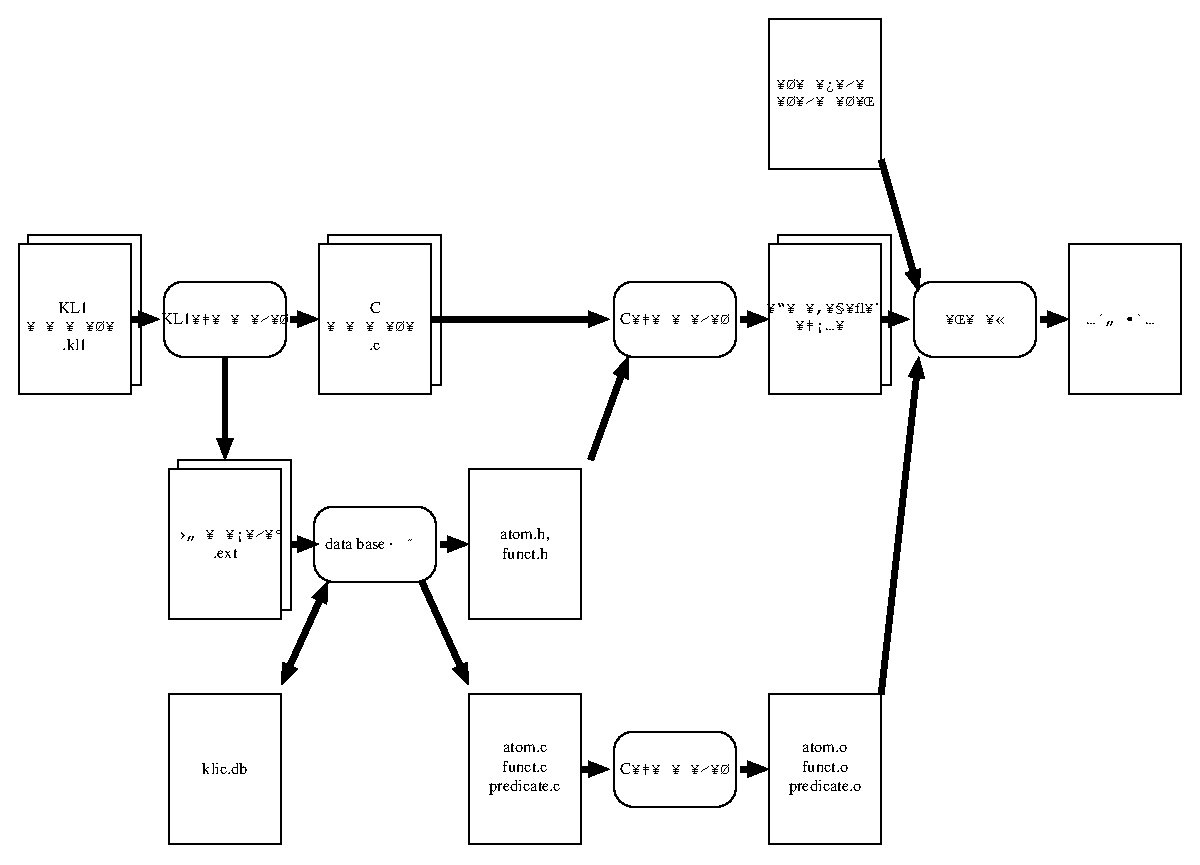
\includegraphics[width=.9\textwidth]{fig/klicflow2.eps}
\end{center}
\caption{klicシステム全体の流れ}
\label{fig:flow2}
\end{figure}

\subsection{コンパイラオプション}
ここまでで\verb|-c|, \verb|-o|, \verb|-v|というオプションを使ったが, 
これら以外にもさまざまなオプションが用意されている.  
表\ref{tab:options}にまとめる.  

\begin{table}
\caption{主なklicコマンドのオプション}
\label{tab:options}
\begin{center}
\begin{tabular}{l||l}
\hline
オプション & 意味\\
\hline\hline
-C & コンパイルのみ (Cソースが出力)\\
\hline
-c & コンパイルのみ (オブジェクトが出力)\\
\hline
-d & 何を実行するかの表示 (実際のコンパイルはしない)\\
\hline
-g & Cコンパイル時にデバッグオプション ({\tt -g}) を付加\\
\hline
-Idirectory & Cコンパイル時のインクルードパス指定\\
\hline
-Ldirectory & リンク時のライブラリパス指定\\
\hline
-lxxx & リンク時のライブラリ指定 (libxxx.aをリンク)\\
\hline
-o executable & 実行ファイルのファイル名指定\\
\hline
-Odigit & Cコンパイラに対する最適化レベル指定\\
\hline
-R & ファイルの依存性を無視して強制再コンパイル\\
\hline
-S & 機械語アセンブラソース出力\\
\hline
-v & verbose mode\\
\hline
-? & ヘルプ\\
\hline
\hline
xxx.kl1 & KL1ファイル名\\
\hline
xxx.c & Cファイル名\\
\hline
xxx.o & objectファイル名\\
\hline
xxx.ext & 記号表ファイル名\\
\hline
\end{tabular}
\end{center}
\vspace*{-12pt}
\end{table}

\section{エラーメッセージ}
\verb|klic|コマンドは, コンパイル対象のKL1プログラムにエラーを
発見すると, エラーを出力する.  
但し, このエラーは, Cコンパイラ, リンカ等で出力されているケースも
ある.  

\verb|klic|コマンドの出力するエラーメッセージは大別すると
以下のようになる.  

\begin{itemize}
\item KL1 $\Rightarrow$ Cコンパイラの出力するもの
$\ldots$ これは比較的分かりやすいエラーメッセージとなっている筈なので, 
読めばその意味はわかるであろう.  

\item Cコンパイラの出力するもの $\ldots$
Cコンパイラが出力するものとして, 今の所, 以下のものがあげられる.  

\begin{itemize}
\item 未定義述語の使用 $\ldots$ 外部モジュールではない 
(``\verb|モジュール名:|''が付加されていない) 述語を呼び出しているが, 
その述語が当該モジュール内に定義されていない場合, 
Cコンパイラが以下のようなメッセージを出力する.  
\footnote{実際には, KLICで利用するCコンパイラにより
出力されるメッセージは異なる.  
ここであげたものはgcc version 2.6.2のものである.  }

\medskip
% \begin{samplebox}
\begin{Verbatim}[frame=single,baselinestretch=0.8]
demo.c: In function `module_demo':
demo.c:29: label `bar_0_ext_interrupt' used but not defined
demo.c:28: label `bar_0_0' used but not defined
C compilation failed for file demo.c
\end{Verbatim}
% \end{samplebox}

これは, 「bar/0という述語がない」ことを意味している.  
\end{itemize}

\item リンカが出力するもの $\ldots$
リンカが出力するものとして, 今の所, 以下のものがあげられる.  

\begin{itemize}
\item 未定義モジュールの利用
\item 外部未定義述語の利用
\end{itemize}
ともに, 以下のようなメッセージを出力する.  

\medskip
% \begin{samplebox}
\begin{Verbatim}[frame=single,baselinestretch=0.8]
ld: Undefined symbol 
   _predicate_bar_xbar_0 
collect2: ld returned 2 exit status
Linkage failed
\end{Verbatim}
% \end{samplebox}

これは, 「barというモジュールがない.  または, barというモジュールにbar/0
という述語がない」ことを意味する.  
\end{itemize}

% \newpage

\section{実行時オプション}
この章の最後に, klic コマンドで生成されたプログラムを実行する時に
指定可能な実行時オプションを表 \ref{tab:eoptions} に挙げる.

\begin{table}[hbt]
\caption{主な実行時オプション}
\label{tab:eoptions}
\begin{center}
\begin{tabular}{l||l}
\hline
オプション & 意味\\
\hline\hline
-t & トレーサ付き実行\\
\hline
-h size& 初期ヒープサイズをワード単位で指定\\
\hline
-H size& 上限ヒープサイズをワード単位で指定\\
\hline
-g & GC 時間の計測指示\\
\hline
-s & サスペンド回数の計測指示\\
\hline
-v & 実行時ルーチンのバージョン表示\\
\hline
-- & ユーザ指定の実行時オプション列の開始\\
\hline
\end{tabular}
\end{center}
\end{table}

もちろんオプション指定の後に実行時プログラムへの引数が指定できる.
引数の取り出しは unix モジュールの argc/1 述語および argv/1 述語を
利用する.  詳しくはマニュアルを参照されたい.


\chapter{KLIC の実行機構とトレーサの使い方}

この章では, KLICの実行機構とトレーサの使用方法について述べる.

\section{KL1のゴールリダクション方式}
\subsection{ゴール書換えモデル}

KL1プログラムの実行は, ゴールをKL1プログラムで定義された規則に従って書
換えることにより行なわれる. 
KLIC処理系では, ゴールはゴールプールと呼ばれる領域におかれ, 
リダクションの実行により生成されるサブゴール群は再びゴールプールに入れられる.
ゴール書換えモデルは, 基本的に図\ref{goalpool}に示すように, 
以下の処理の繰り返しにより実現される.  

\begin{enumerate}
\item ゴールプールからゴールを1つ取ってくる (ゴール呼びだし操作).
\item ゴール引数の値を, ガード部の規則にしたがってチェックする.  
\item チェックに適合した節を1つ選んでそのボディ部を実行し, 生成されたサブゴール群をゴールプールに入れる (リダクション操作).
\end{enumerate}

\begin{figure}[htb]
\begin{center}
% \epsfile{file=goalpool.eps,width=10cm}
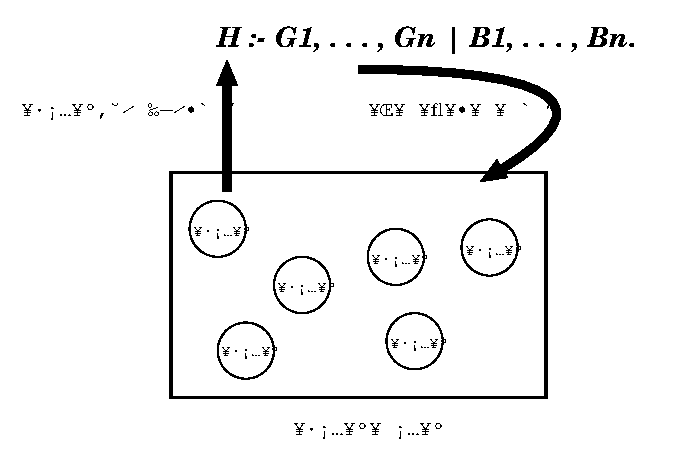
\includegraphics[width=.6\textwidth]{fig/goalpool.eps}
\caption{ゴールプールとリダクション操作}
\label{goalpool}
\end{center}
\end{figure}

\subsection{トレーサを用いたリダクション状況の観測}

KLICのトレーサは, 上記のゴール呼びだし操作やリダクション操作などの, ゴー
ル書換えモデルの各操作をモニターするものである.  トレーサでは, 各操作
をモニターする部分を「ポート」と呼ぶ.

例えば, ゴール呼びだし操作をモニターする部分は「CALLポート」と呼ばれ, 
リダクション操作をモニターする部分は「REDUポート」と呼ばれる.  以下に, 
実際のプログラムをトレースする例を示す.

\subsubsection{プログラムをトレーサ付きで実行する方法}

図\ref{sample-pro1}に例題として, 数を要素とするあるリストが他のリスト
の部分集合となっているか調べるプログラムを示す.   

\begin{figure}[htb]
% \begin{samplebox}
\begin{Verbatim}[frame=single,baselinestretch=0.8]
:- module main.

main :- true | subset(yes, [3,1], [1,3,5], Ans), 
               io:outstream([print(Ans),nl]).

subset(no,  X,    Y,Ans) :- true | Ans = no.
subset(yes, [],   Y,Ans) :- true | Ans = yes.
subset(yes, [A|B],Y,Ans) :- true | member(A,Y,Ans1), subset(Ans1,B,Y,Ans).

member(A, B, Ans) :- B = []            | Ans = no.
member(A, B, Ans) :- B = [X|Y], A =:= X | Ans = yes.
member(A, B, Ans) :- B = [X|Y], A =\= X | member(A, Y, Ans).
\end{Verbatim}
% \end{samplebox}
\caption{部分集合をチェックするプログラム}
\label{sample-pro1}
\end{figure}

%このプログラムを {\tt -t} オプションを付けてコンパイルすると, トレース用のオブジェクトができる.  
%
生成されたオブジェクトプログラムを {\tt -t} オプションを付けて起動し,
{\tt <CR>} を入力し続けると以下に示すように, 実行をトレースできる.  

%\begin{figure}[htb]
%\begin{samplebox}
\begin{quote}
% \begin{quote}
% \begin{samplebox}
\begin{Verbatim}[frame=single,baselinestretch=0.8]
% klic -o subset subset.kl1                                            1
% subset -t
   1 CALL:main:main? 							 
   1 REDU:main:main :-
   2   0:+subset(yes,[3,1],[1,3,5],_3)                                 5
   3   1:+io:outstream([print(_3),nl])? 
   2 CALL:main:subset(yes,[3,1],[1,3,5],_3)? 
   2 REDU:main:subset(yes,[3,1],[1,3,5],_3) :-
   4   0:+member(3,[1,3,5],_11)
   5   1:+subset(_11,[1],[1,3,5],_3)?                                 10
   4 CALL:main:member(3,[1,3,5],_11)? 
   4 REDU:main:member(3,[1,3,5],_11) :-
   6   0:+member(3,[3,5],_11)? 
   6 CALL:main:member(3,[3,5],_11)? 
   6 REDU:main:member(3,[3,5],yes)?                                   15
   5 CALL:main:subset(yes,[1],[1,3,5],_3)? 
   5 REDU:main:subset(yes,[1],[1,3,5],_3) :-
   7   0:+member(1,[1,3,5],_21)	
   8   1:+subset(_21,[],[1,3,5],_3)? 
   7 CALL:main:member(1,[1,3,5],_21)?                                 20
   7 REDU:main:member(1,[1,3,5],yes)? 
   8 CALL:main:subset(yes,[],[1,3,5],_3)? 
   8 REDU:main:subset(yes,[],[1,3,5],yes)? 
   3 CALL:io:outstream([print(yes),nl])? s
yes                                                                   25
% 
\end{Verbatim}
% \end{samplebox}
% \end{quote}
\end{quote}
%\end{samplebox}
%\caption{部分集合をチェックするプログラムのトレース結果}
%\label{trace1}
%\end{figure}

\subsubsection{トレース結果の読み方}

\begin{itemize}\parskip=0mm\itemsep=0.0\baselineskip
\item プログラム中のゴールには通し番号が付けられる.  トレース結果の各
行の最初の数字は, ゴールの番号である.   
\item {\tt 1 CALL:main:main? } (3行目) は, 「main モジュールの main述
語が呼び出された.  」ことを意味する.  つまり, ゴールプールから {\tt
main:main}という述語が取り出されてきたことを意味している.   
\item {\tt 1 CALL:main:main? }が表示された所で, トレーサは入力待ちにな
る.  ここで{\tt <CR>}を入力すると, プログラムを次に進めることができる. 
(?が出ている所ではさまざまなトレーサのコマンドが入力できるが, 詳細は
後で述べる) 
\item 4行目から6行目の
\begin{Verbatim}[baselinestretch=0.8]
       1 REDU:main:main :-
       2     0:+subset(yes,[3,1],[1,3,5],_3)
       3     1:+io:outstream([print(_3),nl])?
\end{Verbatim}
は, main:main が REDUポート を通過し, {\tt subset(yes, [3, 1], [1, 3,
5], \_3)} と {\tt io:\linebreak[1]outstream([print(\_3), nl])} の2つ
のゴールをゴールプールに入れたことを意味する.  KLICのトレーサでは, 具
体値はその値がそのまま表示され, 変数は全て \_で 始まる文字に変換されて
表示される.

\item 7行目の {\tt 2 CALL:main:subset(yes,[3,1],[1,3,5],\_3)?} は, 
前のリダクションでゴールプールに入れられた, ゴール番号 2番のゴールが
呼び出されたことを意味する. 以下, 同様のリダクション操作が続く.

\item 23行目の {\tt 3 CALL:io:outstream([print(yes),nl])? s} では, 
6行目でゴールプールに入れられた, ゴール番号3番のゴールが呼び出されている.
トレースからも分かるように, KLICのゴールプールはLIFOのキューとなっている.

また, この行では{\tt s} というコマンドを入力している.  これは, {\tt
io:\linebreak[1]outstream}というゴールのトレースを行なわないことを意味
する.  {\tt io:\linebreak[1]outstream} は, KL1で書かれているKLICシステ
ムのユーティリティであり, この内部まで詳細にトレースする必要はないから
である.
\end{itemize}

\section{サスペンションメカニズム}

ゴール書換えモデルにおいて, ゴールプールからゴールを1つ取り出し
ゴール引数の値をKL1節のガード部の規則にしたがってチェックしする際に, 
そのチェックがサスペンドする場合は, そのゴールのリダクションは中断され
ゴールはサスペンドゴールプールに入れられる.  
(サスペンド操作)

サスペンドゴールプールに入れられたゴールは, 中断原因となった変数が
具体化されるとゴールプールに移される.  (リジューム操作)

図\ref{fig-suspend}にサスペンドゴールプールを用いたサスペンションメカニズムの
概略図を示す.  

\begin{figure}[htb]
\begin{center}
% \epsfile{file=suspention1.eps,width=10cm}
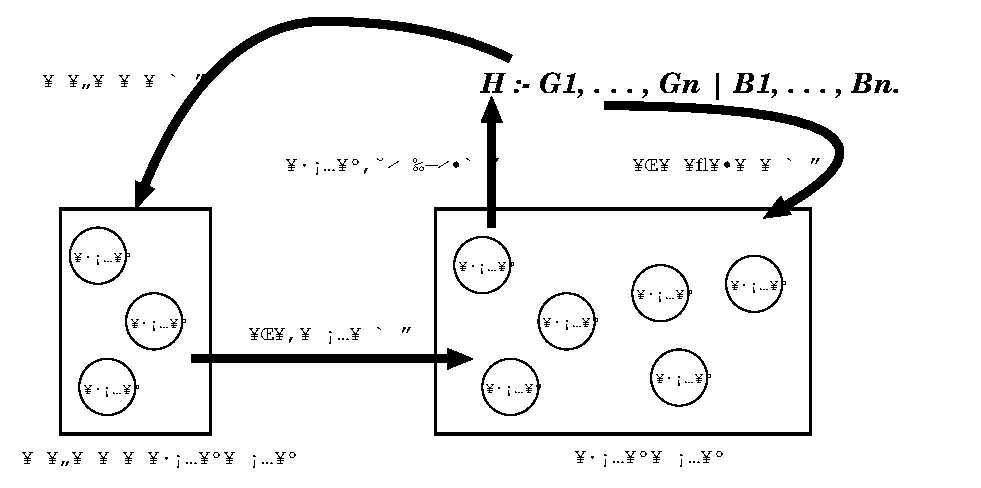
\includegraphics[width=.8\textwidth]{fig/suspention1.eps}
\caption{サスペンションメカニズム}
\label{fig-suspend}
\end{center}
\end{figure}

\subsection*{サスペンドするプログラムのトレース}

図\ref{sample-pro1}のプログラムで, {\tt subset}の第3節を
\begin{verbatim}
subset(yes,[A|B],Y,Ans) :- true | subset(Ans1,B,Y,Ans), member(A,Y,Ans1).
\end{verbatim}
とするとサスペンションが起きる.  

このプログラムのトレース結果を以下に示す.  

%\begin{figure}[htb]
%\begin{samplebox}
\begin{quote}
% \begin{quote}
% \begin{samplebox}
\begin{Verbatim}[frame=single,baselinestretch=0.8]
% klic -o susp susp.kl1                                                1
% susp -t
   1 CALL:main:main? 
   1 REDU:main:main :-
   2   0:+subset(yes,[3,1],[1,3,5],_3)                                 5
   3   1:+io:outstream([print(_3),nl])? 
   2 CALL:main:subset(yes,[3,1],[1,3,5],_3)? 
   2 REDU:main:subset(yes,[3,1],[1,3,5],_3) :-
   4   0:+subset(_13,[1],[1,3,5],_3)
   5   1:+member(3,[1,3,5],_13)?                                      10
   4 CALL:main:subset(_13,[1],[1,3,5],_3)? 
   4 SUSP:main:subset(_13,[1],[1,3,5],_3)? 
   5 CALL:main:member(3,[1,3,5],_63D7)? 
   5 REDU:main:member(3,[1,3,5],_63D7) :-
   6   0:+member(3,[3,5],_63D7)?                                      15
   6 CALL:main:member(3,[3,5],_63D7)? 
   6 REDU:main:member(3,[3,5],yes) :-
   4   0!+subset(yes,[1],[1,3,5],_3)? 
   4 CALL:main:subset(yes,[1],[1,3,5],_3)? 
   4 REDU:main:subset(yes,[1],[1,3,5],_3) :-                          20
   7   0:+subset(_29,[],[1,3,5],_3)
   8   1:+member(1,[1,3,5],_29)? 
   7 CALL:main:subset(_29,[],[1,3,5],_3)? 
   7 SUSP:main:subset(_29,[],[1,3,5],_3)? 
   8 CALL:main:member(1,[1,3,5],_63B8)?                               25
   8 REDU:main:member(1,[1,3,5],yes) :-
   7   0!+subset(yes,[],[1,3,5],_3)? 
   7 CALL:main:subset(yes,[],[1,3,5],_3)? 
   7 REDU:main:subset(yes,[],[1,3,5],yes)? 
   3 CALL:io:outstream([print(yes),nl])? s                            30
yes
%
\end{Verbatim}
% \end{samplebox}
% \end{quote}
\end{quote}
%\end{samplebox}
%\caption{サスペンドするプログラムのトレース例}
%\label{program2}
%\end{figure}

\begin{itemize}\parskip=0mm\itemsep=0.0\baselineskip
\item ゴールがサスペンドする操作をモニターするポートを SUSP ポートと呼
ぶ.  トレースの12行目の, {\tt 4 SUSP: main:\linebreak[1]subset(\_13,
[1], [1, 3, 5], \_3)} は, ゴール番号4番の {\tt
main:\linebreak[1]subset(\_13, [1], [1, 3, 5], \_3)} がサスペンドし
サスペンドゴールプールに入れられたことを意味する.
\item 18行目の, \\
{\tt 4 0!+subset(yes, [1], [1, 3, 5], \_3)}\\は, ゴール番号4番の {\tt
main:subset(\_13, [1], [1, 3, 5], \_3)} がリジュームし, ゴールプールに
移されたことを示す.

\end{itemize}

\section{トレーサの使用方法}

前章でも述べたようにKLICでは, 以下の操作の繰り返しによりリダクションを進める.  

\begin{enumerate}
\item ゴールプールからゴールを1つ取ってくる.  (ゴール呼びだし操作)
\item ゴール引数の値を, ガード部の規則にしたがってチェックし, チェックに適合した節を1つ選んでそのボディ部を実行し, 生成されたサブゴールをゴールプールに入れる.  (リダクション操作)
\item 2 で呼び出されたゴールの引数のチェックがサスペンドする時, ゴール
をサスペンドゴールプールに入れる.  (サスペンション操作)
\end{enumerate}

% \begin{figure}[htb]
% \begin{center}
% \epsfile{file=port.eps,width=10cm}
% \caption{KL1の実行モデルと各ポート}
% \end{center}
% \end{figure}

KLICのトレーサで提供されるポートは, 前述の CALLポート, REDUポート, SUSPポート
と, 後で述べるリダクションの失敗を扱うFAILポートの4つである.  

トレースモードでコンパイルされたプログラムは, ゴールが上記の4つのポート
を通過する時に, 実行を停止してユーザからの入力待ちとなったり, 
そのゴールの表示を行なったりする.  

\subsection{トレーサの出力形式}

%\begin{figure}[htb]
%\epsfile{file=portout1.eps,width=8cm}
%\end{figure}

図\ref{portout}に各ポートでの出力形式を示す.  

\begin{figure}[htb]
\begin{center}
% \epsfile{file=portout1.eps,width=8cm}
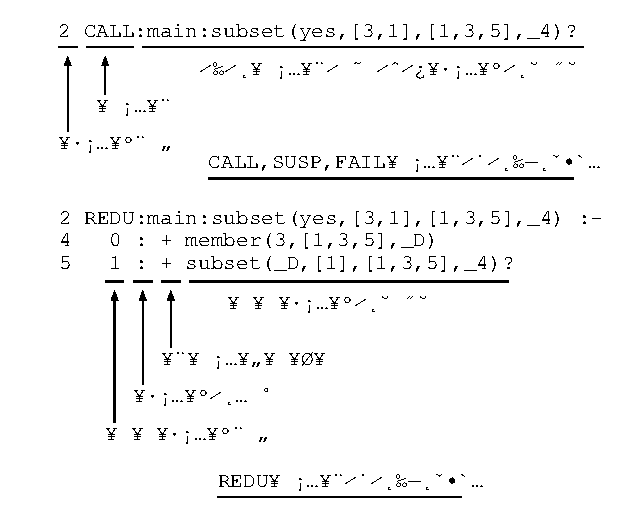
\includegraphics[width=.6\textwidth]{fig/portout1.eps}
\end{center}
\caption{各ポートでの出力形式}
\label{portout}
\end{figure}

CALLポート, SUSPポート, FAILポートでは, ゴール番号, ポート名, 
ゴールレコードの内容が表示される.  
右端の?は, ユーザの入力待ちのプロンプトを意味する.  

REDUポートでは, 先ずリダクションされるゴールがCALLポートと同じ形式で表示され, 
続いて, ゴールプールにエンキューされるゴール群が表示される.  

ゴールプールにエンキューされるゴールは, 
ゴール番号, その節で一意に決まるサブゴール番号, エンキューされるゴールの種別, 
そのゴールのトレースフラグ, サブゴールの内容, の順に表示される.  

エンキューされるゴールの種別は, 以下の4つの記号で示される.  

\vspace{3mm}
\begin{center}
\begin{tabular}{c|c} \hline
ゴール種別 & 意味 \\ \hline
{\tt :}& 通常ゴールのエンキュー\\
{\tt *}& プライオリティつきゴールのエンキュー\\
{\tt !}& 通常ゴールのリジューム\\
{\tt \#}& プライオリティつきゴールのリジューム\\ \hline
\end{tabular}
\end{center}
\vspace{3mm}

トレースフラグは各サブゴールに付けられるフラグで, トレーサはトレースフラグが
{\tt on}であるゴールのみをトレースする.  トレーサはトレースフラグが{\tt on}
ならば{\tt +}を, トレースフラグが{\tt off}ならば{\tt -}を表示する.  
デフォルトでは, 全てのゴールが トレース {\tt on} である.  

\subsection{トレーサの各コマンドの詳細}

{\tt ?}が出力された所で, トレーサはユーザのコマンド入力待ちになる.  
表 \ref{tracer-command}
にコマンドの一覧を示し, 以下に各コマンドの
詳細を述べる.  

\begin{table}%[p]
\begin{center}
\small
\begin{tabular}{l|l|l|l} \hline 
コマンド名 & コマンド入力形式& 入力可能ポート& コマンドの意味\\ \hline \hline
Continue &{\tt <cr>,c}	& 全てのポート 	& 対象となるゴールのトレースを続ける\\ 
Abort& {\tt a}	& 全てのポート 	& 対象となるプログラムのトレースを止める \\ 
Skip&{\tt s}	& 全てのポート & 対象となるゴールのトレースを止める\\
Leap&{\tt l}	& 全てのポート & spyされたサブゴールが現れるまで, \\
	&& &トレースの表示・入力を抑制する\\ 
Enable port&{\tt E} \verb*a a ポート名& 全てのポート& そのポートを観測する\\
Disable port&{\tt D} \verb*a a ポート名& 全てのポート& そのポートは観測しない\\
Leash port&{\tt L} \verb*a a ポート名& 全てのポート& そのポートでユーザからの入力待ちにする\\
Unleash port&{\tt U} \verb*a a ポート名& 全てのポート& そのポートでゴールの表示だけ行なう\\ 
Trace&{\tt +}サブゴール番号 & REDUポート& そのサブゴールをトレース対象とする\\
Notrace&{\tt -}サブゴール番号 & REDUポート& そのサブゴールをトレース対象外とする\\
Toggle trace&サブゴール番号 & REDUポート& そのサブゴールをトレースフラグを反転する\\ 
Notrace default &n \verb*a a述語 & 全てのポート & その述語をトレース対象外とする \\
Trace default&t \verb*a a述語 & 全てのポート & その述語をトレース対象とする \\
Spy&{\tt S} \verb*a a述語 & 全てのポート & その述語にスパイをかける\\
Nospy&{\tt N} \verb*a a述語 & 全てのポート & その述語のスパイを外す\\ 
Set Print Depth&pd \verb*a a引数 & 全てのポート & 表示する構造の深さの変更 \\
Set Print Length&pl \verb*a a引数 & 全てのポート & 表示する構造の長さの変更 \\
Toggle Verbose print&pv      & 全てのポート & verboseモードへの切替え\\
Status query&=	& 全てのポート & 現在のパラメータの状況を表示\\
List Modules &lm	& 全てのポート & 全モジュールの表示\\
List Predicates&lp	& 全てのポート & 全述語の表示\\
Help&h,?	& 全てのポート & 全モジュールの表示\\ 
Queue&Q	& 全てのポート & ゴールプール内のゴールの表示\\ \hline
\end{tabular}
\end{center}
\caption{トレーサのコマンド一覧}
\label{tracer-command}
\end{table}

\subsubsection{実行制御コマンド}

ここでは, トレースを続けたり中止したりするコマンドについて説明する.  

\begin{quote}
\begin{description}
\item[c, $<$cr$>$]  そのままトレースを続行し, 
次のポートで止まり, 再び入力待ちとなる.  

\item[a] トレースを中止する.  
プログラムはその時点から最後までフリーに実行される.  

\item[s] その時点でコマンド入力待ちのポートにあるゴールのトレース
フラグを{\tt off}にする.  新たにトレース{\tt on} となっているゴールが
ポートを通過するまで, プログラムはフリーに実行される.  

\item[l] スパイされたゴールがポートを通るまで, トレースの表示・入力を抑制する.
スパイされたゴールがポートを通ると, トレースモードに戻る.

\end{description}
\end{quote}

また以下のコマンドは, サブゴールのトレースフラグの {\tt on/off}を制御する
もので, REDUポートでのみ入力可能である.  

\begin{quote}
\begin{description}
\item [+ サブゴール番号:] そのサブゴールのトレースフラグを{\tt on}にする.  
\item [− サブゴール番号:] そのサブゴールのトレースフラグを{\tt off}にする.  
\item [サブゴール番号:]   そのサブゴールのトレースフラグを反転する.  
\end{description}
\end{quote}

図\ref{sample-pro1}の部分集合をチェックするプログラムを用いた, 
`{\tt c}', `{\tt <cr>}', `{\tt a}', `{\tt s}' コマンドの使用例を以下に示す.  
`{\tt l}' コマンドはリープコマンドと呼ばれる.  後で述べるスパイ機能と
併せて使用例を示す. 

\begin{quote}% \begin{quote}
\begin{Verbatim}[frame=single,baselinestretch=0.8]
% subset -t                                                          1
   1 CALL:main:main? 
   1 REDU:main:main :-
   2   0:+subset(yes,[3,1],[1,3,5],_3)
   3   1:+io:outstream([print(_3),nl])? c                            5
   2 CALL:main:subset(yes,[3,1],[1,3,5],_3)? 
   2 REDU:main:subset(yes,[3,1],[1,3,5],_3) :-
   4   0:+member(3,[1,3,5],_11)
   5   1:+subset(_11,[1],[1,3,5],_3)? 
   4 CALL:main:member(3,[1,3,5],_11)? s                             10
   5 CALL:main:subset(yes,[1],[1,3,5],_3)? 
   5 REDU:main:subset(yes,[1],[1,3,5],_3) :-
   6   0:+member(1,[1,3,5],_1C)
   7   1:+subset(_1C,[],[1,3,5],_3)? -0
   5 REDU:main:subset(yes,[1],[1,3,5],_3) :-                        15
   6   0:-member(1,[1,3,5],_1C)
   7   1:+subset(_1C,[],[1,3,5],_3)? 
   7 CALL:main:subset(yes,[],[1,3,5],_3)? 
   7 REDU:main:subset(yes,[],[1,3,5],yes)? 
   3 CALL:io:outstream([print(yes),nl])? a                          20
% 
\end{Verbatim}
% \end{quote}
\end{quote}

10行目の `{\tt s}' コマンドにより, ゴール番号4番の member ゴールはトレー
スされなくなった.  14行目の `{\tt -0}' コマンドにより, ゴール番号6番の 
member 述語はトレースされなくなった.  12行目の `{\tt a}' コマンドによ
り, トレースが中止されプログラムが最後まで実行された.

\subsubsection{デフォルトトレースフラグ設定機能}

ある特定の述語を指定して, その述語を実行する全てのゴールのトレース
フラグをデフォルトで設定することができる.  

\begin{quote}
\begin{description}
\item[n 述語] その述語を実行するゴールがデフォルトでトレース{\tt off}となる.  
\item[t 述語] その述語を実行するゴールがデフォルトでトレース{\tt on}となる.  
\end{description}
\end{quote}

述語の指定方法には以下に示す5通りがある.  

\vspace{3mm}
\begin{center}
\begin{tabular}{l|c}\hline
指定方法  &意味\\ \hline
モジュール名:述語名/引数個数 &述語の全情報の明示的な指定 \\
モジュール名:述語名 &指定したモジュールの指定した述語名を持つ全ての述語 \\
モジュール名:&指定したモジュールの全ての述語 \\
述語名/引数個数&実行中モジュール内の指定した述語名と引数個数を持つ述語 \\
述語名&実行中モジュール内で指定した述語名を持つ全ての述語\\ \hline
\end{tabular}
\end{center}
\vspace{3mm}

デフォルトトレースフラグ設定の例を以下に示す.  

\begin{quote}% \begin{quote}
\begin{Verbatim}[frame=single,baselinestretch=0.8]
% subset -t                                                           1
   1 CALL:main:main? 
   1 REDU:main:main :-
   2   0:+subset(yes,[3,1],[1,3,5],_3)
   3   1:+io:outstream([print(_3),nl])? n member                      5
	Default trace reset on predicate main:member/3
   1 REDU:main:main :-
   2   0:+subset(yes,[3,1],[1,3,5],_3)
   3   1:+io:outstream([print(_3),nl])? 
   2 CALL:main:subset(yes,[3,1],[1,3,5],_3)?                         10
   2 REDU:main:subset(yes,[3,1],[1,3,5],_3) :-
   4   0:-member(3,[1,3,5],_11)
   5   1:+subset(_11,[1],[1,3,5],_3)? 
   5 CALL:main:subset(yes,[1],[1,3,5],_3)? 
   5 REDU:main:subset(yes,[1],[1,3,5],_3) :-                         15
   6   0:-member(1,[1,3,5],_1C)
   7   1:+subset(_1C,[],[1,3,5],_3)? 
   7 CALL:main:subset(yes,[],[1,3,5],_3)? 
   7 REDU:main:subset(yes,[],[1,3,5],yes)? 
   3 CALL:io:outstream([print(yes),nl])? s                           20
yes
% 
\end{Verbatim}
% \end{quote}
\end{quote}

5行目で, 述語 {\tt main:member/3}のトレースフラグを{\tt off}に
している.  このことによりそれ以降は, 述語 {\tt main:\linebreak[1]member/3}
のトレースは行なわれない.  

\subsubsection{スパイ制御機能}
スパイ制御機能コマンドを以下に示す.  

\begin{quote}
\begin{description}
\item [S 述語] 指定した述語にスパイを掛ける.  
述語名を指定しないと, 現在トレースしている述語にスパイが掛かる.  

\item [N 述語] 指定した述語のスパイを外す.  
述語名を指定しないと, 現在トレースしている述語のスパイが外れる.  
\end{description}
\end{quote}

実行制御コマンドで説明した `{\tt l}' コマンドは, スパイされたゴールが
ポートを通るまで, トレースの表示・入力を抑制する.

このため, スパイ機能と `{\tt l}' コマンドを組合わせて使うと, ある特定
の述語だけにトレースを掛けてデバッグを進めることができる.

以下にスパイと `{\tt l}' コマンドの使用例を示す.  

\begin{quote}% \begin{quote}
\begin{Verbatim}[frame=single,baselinestretch=0.8]
% subset -t                                                            1
   1 CALL:main:main? S member
	Spy point set on predicate main:member/3
   1 CALL:main:main? l
   4 CALL:main:member(3,[1,3,5],_11)?                                  5
   4 REDU:main:member(3,[1,3,5],_11) :-
   6   0:+member(3,[3,5],_11)? 
   6 CALL:main:member(3,[3,5],_11)? 
   6 REDU:main:member(3,[3,5],yes)? 
   5 CALL:main:subset(yes,[1],[1,3,5],_3)?                            10
   5 REDU:main:subset(yes,[1],[1,3,5],_3) :-
   7   0:+member(1,[1,3,5],_21)
   8   1:+subset(_21,[],[1,3,5],_3)? 
   7 CALL:main:member(1,[1,3,5],_21)? 
   7 REDU:main:member(1,[1,3,5],yes)? N member                        15
	Spy point reset on predicate main:member/3
   7 REDU:main:member(1,[1,3,5],yes)? 
   8 CALL:main:subset(yes,[],[1,3,5],_3)? 
   8 REDU:main:subset(yes,[],[1,3,5],yes)? 
   3 CALL:io:outstream([print(yes),nl])? s                            20
yes
% 
\end{Verbatim}
% \end{quote}
\end{quote}

2行目で, 述語 {\tt main:member/3}にスパイを掛けている.  
3行目のゴール{\tt main:main}において, `{\tt l}' コマンドを実行することにより, 
{\tt main:member/3}を実行したところからトレースが始まる.  

\subsubsection{ポートの制御}

ここでは, ポートでの入出力を制御するコマンドについて述べる.  

ポート制御コマンドは, `コマンド\verb*a aポート名'の形式で入力する.  
ポート名の指定方法は以下に示す通りである.  

\vspace{3mm}
\begin{center}
\begin{tabular}{l|l} \hline
ポート名 & 指定方法 (大文字, 小文字の区別なし) \\ \hline
CALLポート & c, call \\
REDUポート & r, redu, reduce \\
SUSPポート & s, susp, suspend \\
FAILポート & f, fail \\
全ポート   & a, all\\ \hline
\end{tabular}
\end{center}
\vspace{3mm}

またポート制御コマンドには, 以下の4つがある.  
\begin{quote}
\begin{description}
\item[D~~ポート名] 対象となるポートでのトレースを行なわない (ポートを Disable 状態にする.)

\item[E~~ポート名] 対象となるポートでの表示・入力を再開する (ポートを Enable 状態にする.)

\item[U~~ポート名] 対象となるポートでは表示のみを行ない, 入力待
ちにならない (ポートを Unleash 状態にする.)

\item[L~~ポート名] 対象となるポートでコマンド入力待ちになる (ポートを Leash 状態にする.)

\end{description}
\end{quote}

デフォルトでは, 全てのポートが Enable状態, Leash状態である.  各コマンドの使用例を以下に示す.  

\begin{quote}% \begin{quote}
\begin{Verbatim}[frame=single,baselinestretch=0.8]
% subset -t                                                            1
   1 CALL:main:main? U redu
   1 CALL:main:main? 
   1 REDU:main:main :-
   2   0:+subset(yes,[3,1],[1,3,5],_3)                                 5
   3   1:+io:outstream([print(_3),nl])
   2 CALL:main:subset(yes,[3,1],[1,3,5],_3)? 
   2 REDU:main:subset(yes,[3,1],[1,3,5],_3) :-
   4   0:+member(3,[1,3,5],_11)
   5   1:+subset(_11,[1],[1,3,5],_3)                                  10
   4 CALL:main:member(3,[1,3,5],_11)? L redu
   4 CALL:main:member(3,[1,3,5],_11)? 
   4 REDU:main:member(3,[1,3,5],_11) :-
   6   0:+member(3,[3,5],_11)? 
   6 CALL:main:member(3,[3,5],_11)? D call                            15
   6 CALL:main:member(3,[3,5],_11)? 
   6 REDU:main:member(3,[3,5],yes)? 
   5 REDU:main:subset(yes,[1],[1,3,5],_3) :-
   7   0:+member(1,[1,3,5],_21)
   8   1:+subset(_21,[],[1,3,5],_3)? a                                20
yes
%
\end{Verbatim}
% \end{quote}
\end{quote}

2行目でREDUポートをunleashしているので, 8-10行目のREDUポートでは, 
ユーザの入力待ちにならない.  
その後, 11行目でREDUポートをleashしたので, 13行目以降はREDUポートで
入力待ちになった.  
15行目でCALLポートをdisableしているので, 以下のトレースではCALLポートの
トレースは表示されない.  

\subsubsection{その他補助機能}

その他, 以下のトレース環境の設定・表示機能がある.  

\vspace{5mm}
\begin{tabular}{ll}
{\bf pd \it dep}&  表示する構造の深さを `{\it dep}' に設定する.   \\
{\bf pl \it len}&  表示する構造の長さを `{\it len}'に設定する.   \\
{\bf pv}&  verboseモードフラグのトグルを行なう.  \\
	&   verboseモード{\tt on}状態では, ゴールをサスペンドさせている変数が\\
	& 表示される際に, そのゴールも一緒に表示される.  \\
{\bf =}	&  現在のパラメータの状況を表示する.  		\\
{\bf lm}&   プログラムを構成している全モジュールを表示する.  		\\
{\bf lp}&	プログラムを構成している全述語を表示する.  		\\
{\bf Q} & ゴールプール内のゴールを全て表示する.  \\
{\bf h} &	  ヘルプ画面を表示する.  			\\
{\bf ?} &	  {\tt h}コマンドと同じ.  			\\
\end{tabular}
\vspace{5mm}

\section{実行時エラーの表示とトレース}

\subsection{節の失敗 (failure)}

呼び出されたゴールを, ガード部の規則にしたがって
チェックしたが, どの節の条件にもマッチしなかった時は, そのゴールは失敗する.  
以下に失敗するプログラムの例とその実行トレースを示す.  

\begin{quote}% \begin{quote}
\begin{Verbatim}[frame=single,baselinestretch=0.8]
:-module main.

main:- true | gen(X), con(X).

gen(X):- true | X = a.

con(b):- true | true.
con(c):- true | true.

% g_fail -t                                                        1
   1 CALL:main:main? 
   1 REDU:main:main :-
   2   0:+gen(_4)
   3   1:+con(_4)?                                                 5
   2 CALL:main:gen(_4)? 
   2 REDU:main:gen(a)? 
   3 CALL:main:con(a)? 
!!! Reduction Failure !!!
   4 FAIL:main:con(a)? a                                          10
% 
\end{Verbatim}
\end{quote}% \end{quote}

節が失敗したため10行目に失敗した節{\tt 4 FAIL:main:con(a)?}が表示された.  
この時は図のように, `{\tt a}' コマンドでトレースを中止することが推奨される.

\subsection{永久中断}

あるゴールがサスペンドしたが, その変数が具体化されないまま
ゴールプールが空になると, 永久中断状態となる.  

以下に永久中断するプログラムの例と実行トレースを示す.  

\begin{quote}% \begin{quote}
\begin{Verbatim}[frame=single,baselinestretch=0.8]
:-module main.

main:- true | gen(X),con(X).

gen(X):- true | true.

con([A|B]):- true | true.

% psus -t                                                           1
   1 CALL:main:main? 
   1 REDU:main:main :-
   2   0:+gen(_4)
   3   1:+con(_4)?                                                  5
   2 CALL:main:gen(_4)? 
   2 REDU:main:gen(_4)? 
   3 CALL:main:con(_4)? 
   3 SUSP:main:con(_4)? 
1 perpetually suspending goals found
!!! Perpetual Suspention Detected !!!
   3 PSUS: main:con(_B)? a
%
\end{Verbatim}
\end{quote}% \end{quote}

ゴール番号3番の {\tt main:con(\_4)}が
サスペンドするが, リジュームされないので永久中断した.  
このため, 10行目に{\tt !!! 1 suspending goal(s) !!!}と表示された.  

\chapter{KLICのインストール法}

この章では, KLICシステムのインストール方法について説明する.  

\section{KLICのコンパイル方式}

まず, インストール法の理解のため, KLICシステムが
KL1 プログラムをどのようにコンパイルして実行するのかを説明する.  

システムは以下のみっつのモジュールからなる.  

\begin{itemize}
\item KLIC コンパイラ

\item KLIC データベース管理

\item KLIC 実行時システム
\end{itemize}

KL1 のプログラムは KLIC コンパイラで C プログラムに翻訳される.  その
時に ``ファイル名.ext''という名の, プログラム中に出てくるアトムやファン
クタの情報を持つファイルも出力する.  後にデータベース管理プログラム
が, 一緒にリンクするプログラムの ``.ext'' ファイルの情報を統合して,
``atom.h'', ``funct.h'', ``atom.c'', ``funct.c'', ``predicates.c'' の
諸ファイルを作成する.

次に, コンパイル結果の C プログラムを C コンパイラで, KLIC システムの
提供するヘッダや ``atom.h'', ``funct.h'' と共にコンパイルする.
``atom.c'', ``funct.c'', ``predicates.c'' のファイルもコンパイルし, 実
行時システムとリンクして実行可能ファイルを作成する.

コンパイル, データベース管理, リンクの一連の作業は ``klic'' という名のド
ライバプログラムが制御する.  この ``klic'' は ``cc'' と ``make'' を合わせ
たような役目を果たす.  ``Cc'' は C のプリプロセサ, コンパイラ本体, 
リンカを制御するが, ``klic'' は KL1 から C へのコンパイラ, C コンパイ
ラ, データベース管理プログラム, そしてリンカを制御する.  ``Make'' はファ
イルの日付を調べて必要なコンパイルだけを行なうが, ``klic''も同様の機能を持つ.  

\section{必要とする環境}
KLICはその部分毎に各々以下のようなソフトウエア環境を必要とする.  

\begin{itemize}
\item KLICコンパイラ $\ldots$
これはKL1自身で書かれている.
KLICの配布キットにはこれを既にCにコンパイルしたコードが含まれている.

\item KLIC実行時システム $\ldots$
これはCで書かれている.  
ANSI Cコンパイラ, さらにGNU Cコンパイラであればより効率のよいコードが
出力されることを念頭に書かれいるが, K\&Rコンパイラであっても
問題なく利用できる.

\item KLICデータベース管理 $\ldots$
これもKLIC実行時システムと同様Cで書かれている.  

\end{itemize}

また, オペレーティングシステムとしては通常のUNIX (Berkeley版, ATT版を
問わず) であれば, 動作することを念頭に書かれている.  

\section{インストール方法}
KLICシステムのインストールは以下のように行なう.  

\subsection{システムの入手}
まず, KLICシステムのソースコードを入手する.  
最も手軽な方法は, ICOTのIFS (ICOT Free Software) アーカイブ 
(ftp.icot.or.jp) より
匿名ftpする方法である.  
この際, ftp を binary (image) mode にすることを忘れずに.  

\subsection{展開}
入手したシステムをディレクトリに展開する必要がある.  
展開のためには, 展開を行なう先のディレクトリ (このディレクトリを以下では
KLICDIRと呼ぶ) で, 
zcat, uncompress, tarなどを使って行なう.  

% \begin{samplebox}
\begin{Verbatim}[frame=single]
% zcat ``ftpしてきたファイル'' | tar xf -
\end{Verbatim}
% \end{samplebox}

この結果, 全てのファイルはディレクトリKLICDIR以下に展開される.  

\subsection{コンフィギュレーション}
KLICをインストールするシステムに合わせて, システムの
パラメタなどを設定する.  このためにはシェルスクリプトKLICDIR/Configure
を走らせて, 会話的に質問に答えていけば良い.  種々のライブラリ関数など
が利用できるかどうかも自動的に判定するようになっている.

コンフィギュレーション・スクリプトへの応答は, 大部分の項目については通
常デフォルト値で良いが, 特に注意すべき項目として, 以下のものがある.
\begin{itemize}
\item
並列処理系のインストールを行なうかどうか.  並列処理系のインストールに
は並列処理ライブラリなどの環境設定が必要である.  最初は並列処理系はイ
ンストールしないことを奨める.  この文書では並列処理系のインストールに
ついてまでは触れない.
\item
非同期入出力のためのレディ・シグナルが使えるかどうか.  これはシステム
に依存するが, ソケットの非同期入出力を利用しないのなら『使えない』と答
えておいてもよい.
\item
インストール先のルートとなるディレクトリ.  デフォルトは``/usr/local''
としているが, システム管理者以外の場合は適当な自分のディレクトリを指定
する.  多くの場合ホームディレクトリを指定すれば良い.
\end{itemize}
コンフィギュレーションの結果, 以下のファイルが生成される.
\begin{verbatim}
      KLICDIR/Makefile
      KLICDIR/include/klic/config.h
\end{verbatim}

\subsection{コンパイル}
KLICDIRで, \verb|make|コマンドによりコンパイルする.  

% \begin{samplebox}
\begin{verbatim}[frame=single]
% make
\end{verbatim}
% \end{samplebox}

これによってコンパイラのドライバ, KL1からCへのコンパイラ, データベース
管理プログラム, 実行時システムのコンパイルが行なわれる.

ここでエラーがおきた場合には設定に問題がある可能性があるので, 
もう一度コンフィギュレーションが正しく行なったか確認すること.  

\subsection{確認}
KLICシステムが正しくコンパイルされたかどうか, 
テストプログラムを実行することで確認できるようになっている.  
KLICDIRで``make tests''とすることで, 基本的なテストプログラムが
コンパイル, 実行され, 結果が確認される.  

% \begin{samplebox}
\begin{Verbatim}[frame=single]
% make tests
\end{Verbatim}
% \end{samplebox}

\subsection{インストール}
ここまで問題なければ, KLICシステムは正しく作成されているので, 
トップディレクトリで``make install''とすることにより, 
Makefileで指定したディレクトリに必要なファイルをコピーする.  
これでインストール終了である.  

% \begin{samplebox}
\begin{Verbatim}[frame=single]
% make install
\end{Verbatim}
% \end{samplebox}

\subsection{掃除}

インストール後にインストール用に作った作業ファイルなどを消去するには以
下を行なう.

% \begin{samplebox}
\begin{Verbatim}[frame=single]
% make distclean
\end{Verbatim}
% \end{samplebox}

\section{トラブルが起きたら}
トラブルがおきた際には, 以下にメールで問い合わせを.  

\begin{quotation}
klic-bugs@icot.or.jp
\end{quotation}

問い合わせの際には以下の情報を添付していただければ, 問題の迅速な解析に
役立つだろう.
\begin{itemize}
\item
使用システムの機種, OSと版名.
\item
Makeのログ.
\item
コンフィギュレーションの結果. すなわち以下のファイルの内容.
\begin{verbatim}
      KLICDIR/Makefile
      KLICDIR/include/klic/config.h
\end{verbatim}
\end{itemize}


\appendix
\chapter{簡易並列実装版の使い方}
本章は, 現在 (1995 年 9 月現在) リリースされている簡易並列版の
使い方について説明する.  なお {\bf 内容は非常に暫定的なものが多いの
で, 実際に使用される際はマニュアルを読み直す必要がある}.

KLIC の 2 種類の並列実装が、配布される KLIC に含まれている.  
このうち現在の配布に含まれる分散メモリ実装と呼ばれる方式には
PVM3.3 を利用した版が存在し, これは簡易並列実装版とも呼ばれ, 同種のマ
シンがネットワーク結合された分散環境でも利用することができる.  この
版の簡単な利用法について説明したいと思う.

この版は PVM に基づいているが, 異種構成をサポートしてない.  
複数のアーキテクチャを持つプロセッサで構成されるシステムや, 異なるオペ
レーティング・システムを動かすシステムでは機能しないことに注意されたい.

\section{分散 KLIC 向けプログラムのコンパイル}
コンパイル手続きは, 以下に示すオプションが利用できる他は, 逐次版とほぼ
同じである.  

\begin{tabular}{lp{10cm}}
-dp&
分散 KLIC システムを用いたコンパイルを指定します.  
このオプションの指定がない場合, コンパイルされるオブジェクト・コードは, 
逐次処理でしか動きません. \\
\end{tabular}

なお {\tt -dp} の代わりに {\tt -shm} オプションを付けると共有メモリ並
列実装版向けのコードが生成される.

\section{分散 KLIC のプログラム実行}

\subsection{PVM のセット・アップ}

分散実行用にコンパイルされたプログラムを実行する前に,  PVM システムが
システム上で稼働している必要がある.  

\subsubsection{分散 KLIC の実行時オプション}

分散 KLIC システムでプログラムを動かす場合, 逐次版で利用できるオプショ
ンに加えて, 以下のオプションが利用できる.   

\begin{tabular}{llp{10cm}}
-p&N&
プログラムを動かすための疑似プロセッサ( Unix プロセス)の数を指定する.  \\
-e&&
バッチ転送モードに切り替える.  
通常,  KLIC は要求時にプロセッサ間でデータ構造を転送する.  
ネストしたデータ構造は通常, 1 度に 1 レベルずつ転送する.  
バッチ転送では, ネストしたデータ構造を 1 度に転送する.  
これをモードでは, ある種のプログラムはより効率的に実行する.  
しかし, 別のプログラムでは性能を劣化させることもある.  \\
-n&&
実行時の統計情報を表示する.  \\
\end{tabular}

\section{ランタイムモニタを使った実行}

並列プログラムの開発では, デバッギングの他チューニングも必要となる.
プログラムのチューニングのためにビジュアルにノードの稼働状況を見る
ツールは非常に威力を発揮する.  そのために KLIC ではランタイムモニタと
呼ばれるツールを用意する.  このツールの利用方法について簡単に
述べる.

\subsection{ランタイムモニタの起動}

ここでは PVM を利用したランタイムモニタについて説明する.  
起動は次の通り.

\begin{Verbatim}
        klicmon 最大ノード数
\end{Verbatim}

すると図 \ref{rmon-empty} のウインドウが表示される (図の場合は,
ノード数 12 とした).  この時 rmonitor の PVM におけるタスク ID を
覚えておくこと.

\begin{figure}[htb]
\begin{center}
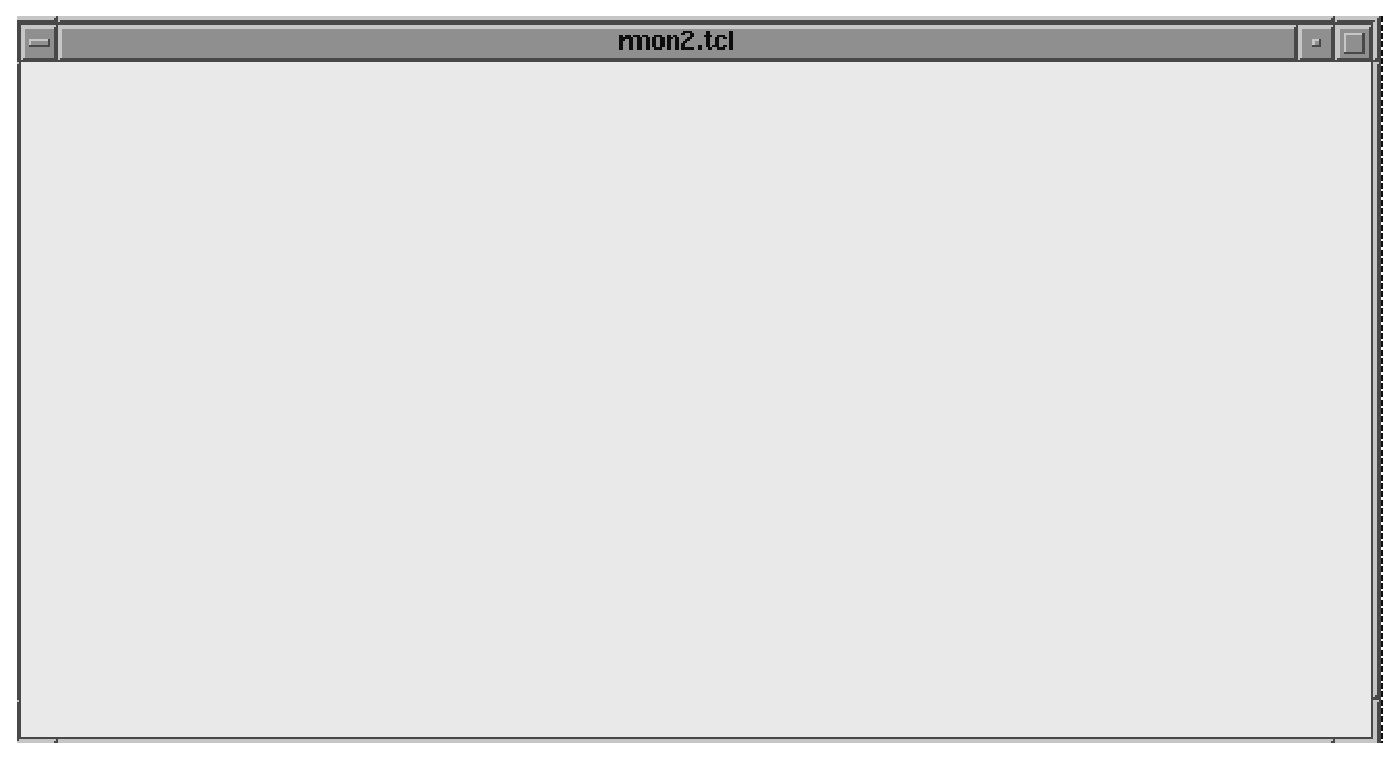
\includegraphics[width=.8\textwidth]{fig/rmon5.ps}
\end{center}
\caption{ランタイムモニタの初期状態}\label{rmon-empty}
\end{figure}

\subsection{ランタイムモニタの利用}

ランタイムモニタを利用する.  例えば {\bf a.out} をノード数 
12 で実行したとする.  またランタイムモニタの PVM における
タスク ID が 40004 とする.  {\bf a.out} を以下の通り実行することで
各ノードの稼働状況が図 \ref{rmon-exec} のように見ることができる.

\begin{Verbatim}
        a.out -p 12 -rmon 40004
\end{Verbatim}

\begin{figure}[hbt]
\begin{center}
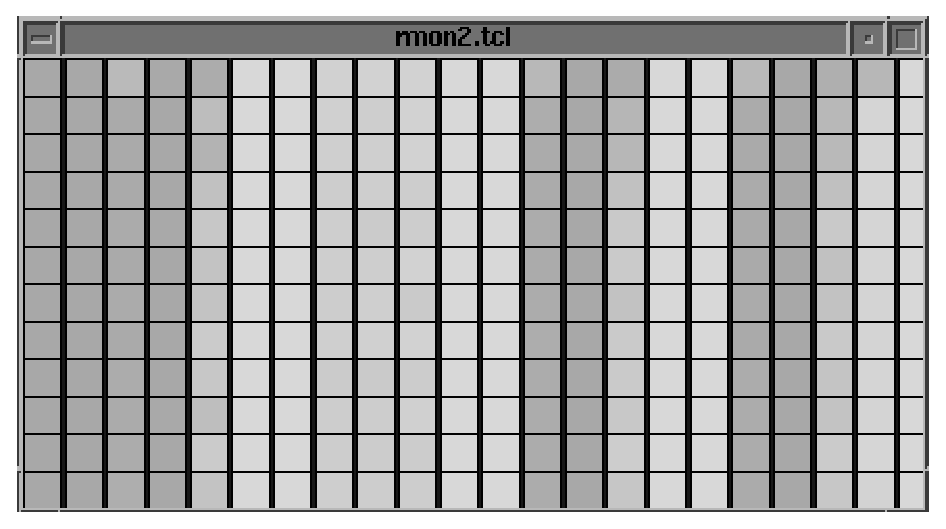
\includegraphics[width=.8\textwidth]{fig/rmon3.ps}
\end{center}
\caption{稼働状況の表示}\label{rmon-exec}
\end{figure}

この図の横軸は右方向への時間軸となる.  画面が一杯になった
場合は, 横スクロールが起こる.  縦軸は各ノードを示す.  
上から下に昇順に並ぶ.

\section{分散 KLIC の既知のバグ}
\begin{itemize}
\item
新しく登録されたアトムとファンクタは, プログラムの実行中に, 正常に処理
されないことがある.  

\item
スパイの指定は, 
指定した計算ノードの内部だけに効果がある.  

\item
永久中断ゴールの検出は行なってない.

\item
PVM は版によってはハングアップすることがある. 念のため PVM のコンソー
ルから稼働しているかどうかを時々確認して欲しい.

\end{itemize}

\end{document}
